\section{Introduction}
For the purposes of this paper, we current define usage management as the management of the usage of resources (and data) across and within computing environments.  More than access control or digital rights management, usage management concerns itself with fine-grained control of all aspects of how a given digital resource is used.  As digital environments become more open over time, the need for usage management for resources that span utility computational environments (e.g. cloud provider systems) will become increasingly important.

With the advent and widespread use of cloud computing, those responsible for a given usage managed resource are almost never those responsible for the computing systems, except at edge devices like mobile phones or other small profile computing devices.  Resources are regularly moved across national boundaries and regional areas without either the content owner's or creator's knowledge.  Furthermore, this kind of transfer is generally according to pre-established algorithms or data routing protocols over which users of all stripes have no control.  Managing these kinds of issues requires new usage management capabilities that can run on platforms ranging from small, hand-held devices to nodes in large data centers.

Historically research in this area has been focused on developing more expressive policy languages via either different type of mathematical logics or formalisms with greater reasoning capabilities~\cite{ArHu:07,BaMi:06,ChCoEtHaJoLa:03,HaWe:04,HaWe:08,PuWe:02,XiBjFu:08}.  These approaches however fail to address interoperability challenges posed by new commercially available distributed computing environments.Interoperability efforts have resorted to translation mechanisms, where the policy is translated in its entirety to a different language~\cite{HeJa:05,PoPrDe:04,ScTaWo:04}; it has been shown recently however that such techniques are infeasible and hard to perform for most policy languages~\cite{KoLaMaMi:04, SaShUe:04}. Other approaches have led to complex policy specification languages that have tried to establish themselves as the universal standard~\cite{OMADRM,ODRL-req,Wa:04,XrML-spec}.  This unfortunately tends to stifle both innovation and flexibility~\cite{HeJa:05,JaHe:04,JaHe:08,JaHeMa:06}.

To address these issues, we first applied the principles of system design to develop a framework for usage management in open, distributed environments that supports interoperability. These principles have been used by researchers in large network design create a balance between interoperability and open, flexible architectures~\cite{Al:04,BlCl:01,ClWrSoBr:02}, allowing for computing scale and power without sacrificing innovation. Initially we standardized certain features of the framework operational semantics, and left free of standards features that necessitate choice and innovation.

We have implemented this framework, including a usage management calculus providing a platform usage management, within a Domain Specific Language (DSL) and associated evaluation environment. The DSL and its environment implements our previously defined framework, separating various roles needed for distributed policy creation and management, provides the capability to develop executable licenses, and is extensible from both a policy and constraint definition perspective.

In this paper, we will first review the problems in usage management in more detail.  Then, in Section \ref{sec:model} we will first review the model we developed to guide the DSL's syntactic and semantic development.  Then, in the next section, we will cover the language itself, how it was developed, and its supporting evaluation environment.  We will then close the paper with three specific implemenation examples showing how the language and its runtime support usage management scenarios from three different environments --- creative commons (CC), the extensible rights markup language (XRML), and the open digital rights language(ODRL).

\section{Motivation}\label{sec:motivation}
Usage management, is a term we have coined in order to describe the management of resource usage within a given system.  In this section we first lay out the historical development of usage management followed by the scope and constituent elements of usage management, tracing its origins to access control and digital rights management . Following this, we explain the challenges that result from the evolving nature in which information is being used across systems. 

\subsection{Access Control}
Access control mechanisms are systems that manage controlled access to resources. The central idea behind access control is that access to a resource is granted depending upon subject attributes, object attributes, and system attributes. The central component of any access control system, is an access control language (ACL) that is used to express rules for granting access to different resources in the system.

Access control policies can be categorized into two types, namely, discretionary access control (DAC) and mandatory access control (MAC)~\cite{HuFeKu:06}. DAC policies are  the policies that are specified by the owner of the resource, based on the users' attributes. On the other hand MAC policies are made by a central authority and apply to the whole system.  A number of access control models have been developed that allow different types of access control in these two modes. The most successful ones being the role-based access control model (RBAC), and the Bell and LaPadula model~\cite{BL:73,BL:76}. The focus of access control models is to capture the different types of relationships between and among a set of resources and a set of users, and express access rules based on those relationships. 

Access control mechanisms are generally tightly coupled with the system in which they are deployed. In situations where users identities are not known apripori, a system agnostic authentication mechanism, such as the public key infrastructure, is used. 

\subsection{Digital Rights Management}
Digital rights management (DRM) consists of mechanisms that manage controlled usage of digital resources. The central idea behind DRM is that usage rules for a given resource are specified for a particular user or group of users, and the use of the resource is subsequently managed for a finite period of time.  The usage rules generally include a set of permissions and obligations, along with rules specifying how the permissions may be exercised over a period of time and under what circumstances. DRM also includes mechanisms such as trusted computing that ensure the enforcement of rights on the user machines~\cite{SaSt:04}. The most well known, but unsuccessful, approaches to address this problem are IBM's Cryptolope and Microsoft's Palladium technologies~\cite{CaJuPoLe:02,IBM:02,KoLoKa:97}.  Given the problem of enforcing DRM, researchers have proposed incentive based, game-theoretic approaches for DRM~\cite{HeJaKhHr:07,ZhPeMaYaHa:09}. The central component of DRM systems is a rights expression language (REL) that is used to express usage rules (or rights) in the form of a license that is generated by a resource owner for a user or a group of users that will use a resource.  

Some of the earliest attempts at DRM date back to 1980's, and involve the development a formal language for legal discourse~\cite{Bo:88,McG:88,McC:89}. At present, creative commons, along with two XML-based RELs, namely, XrML and ODRL, are most commonly used~\cite{XrML:02,Ia:00}. Both XrML and ODRL have formed alliances with major players in the industry and standards bodies.  Semantics of these XML-based languages are informal. A number of approaches using various types of formalisms and approaches have be used to develop formal RELs. Gunter et al.~\cite{GuWeWr:01} and Pucella et al.~\cite{PuWe:02} have used trace-based semantics to develop formal RELs. Other formalisms such as first-order logic and CafeOBJ have been used to develop RELs~\cite{ArHu:07,ChCoEtHaJoLa:03,XiBjFu:08}. Many researchers have attempted to provide formal semantics for existing XML based RELs~\cite{HaWe:04,PuWe:06,HaWe:08}. It is however the general agreement that popular XML-based RELs are difficult to formalize in their entirety~\cite{HaWe:04,HaWe:08,JaHeMa:06}. ,

More recently, researchers have tried to expand the the concept of DRM to propose concepts including usage rights management and usage control. The idea of usage rights management is developed along the lines of making users aware of how a resource is supposed to be used~\cite{HuPaGr:09}. A more formal framework, $UCON_{ABC}$ encompassing usage rules and access control is proposed by Park et al.~\cite{PaSa:04}.

\begin{figure}[t]
 \centerline{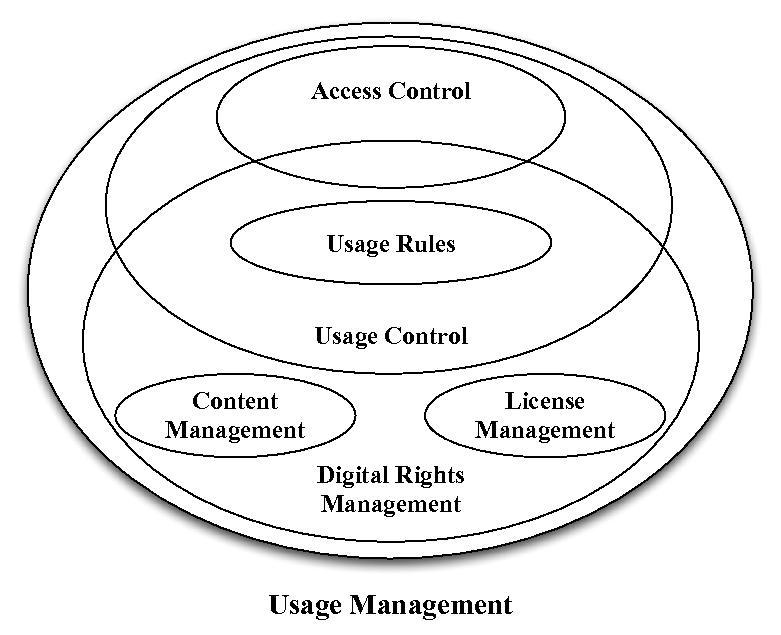
\includegraphics[width=3.5in]{usage_management}}
 \caption{The primary elements in a usage management system.} \label{UM}
\end{figure}


\subsection{Scope of Usage Management}
Before we discuss the scope and components of usage management, it is important to note the difference between ACLs and RELs. Even though the goals of these two types of languages overlap, the focus of research in ACLs and RELs is significantly different.  ACLs focus on defining access rules in terms of relationships between set of resources and set of users. In DRM systems, once a user obtains a license for a resource, access to that resource is implicit, and what matters is how that resource is used from that point onwards. Therefore, RELs  focus on defining different types of usage rules for a given user (or group of users) over a given resource (group of resources). 

We introduce the concept of usage management that is built upon the term {\em usage control} introduced by Park et al.~\cite{PaSa:04}. The usage control model, called  $UCON_{ABC}$, is based on {\em Authorizations, oBligations and Conditions}~\cite{PaSa:04}. $UCON_{ABC}$ combines access control and  permissions and obligations in a single model. 

We now describe the components of usage management as shown in Figure~\ref{UM}, and how they relate to each other. Usage management is a combination of usage control and DRM.  Usage control is a combination of access control and usage rules. Digital rights management includes content management, license management, specification of usage rules and a simplified subset of access control.  Content and license management include processes that manage how content and license are bundled, encrypted and distributed or managed across multiple clients. These processes include encryption mechanisms, trust management, trusted computing platforms and other such management techniques. Many RELs, including XrML and ODRL, have tried to incorporate these functionalities. 

Next, we discuss challenges in implementing usage management systems, and the need for an actionable framework for addressing the challenges. 

\subsection{Challenges in Usage Management}
Unlike classical access control systems, information is increasingly used across highly networked, distributed computing environments that are not a part of a single centrally managed system.  In addition, digital information is increasingly used in innovative ways in which it is transformed, processed or merged with other information while being used across computing environments. One such example is the mashup process where information from two separate sources is merged to generate a new information source. This necessitates usage management policies to be tightly coupled with the resource, rather than the system. The policy is then interpreted and enforced as the resource moves across different computing environments. 

A logical approach to this problem is to build an interpreter for the policy language that runs on the computing environment (or the client), and enforces the policy on the client. This approach has been very successful for access control systems, because access control policies are tightly coupled with computing environments whose nature is known apriori.  However, in usage management scenarios where resources move across environments that are not known apriori, such an approach is infeasible. To address such a situation, each of the computing environments must  incorporate an interpreter and enforcement mechanism that is custom built for different policy languages. 

One of the solutions to this situation is the use of a standard usage policy language for all types of information management ecosystems. Rights expression languages such as XrML and ODRL have been adopted separately as standards by different industry alliances. The semantics of these XML-based languages are informal, and researches have demonstrated the difficulty involved in providing formal semantics for these languages~\cite{HaWe:08}. 

At the same time, numerous formal logic-based rights expression languages have been developed by academicians. These languages use different types of mathematical logics to express and reason over various types of usage semantics. Both XrML and ODRL have developed and continue to develop independent of these formal languages, and have not been able to incorporate their expression and reasoning power.  Hence, unlike formal access control models, these formal languages continue to remain outside the radar of industry alliances. 
 
As a result, none of these languages are likely to become the {\em defacto} industry standard in the future.  Different information ecosystems will continue to use different policy languages according to the policy expression requirements. Such a fragmented use of policy languages will remain the biggest obstacle to achieving usage management along with unhindered flow of information across highly distributed computing environments. Existence of multiple policy languages in such scenarios pose two problems, namely, difficulty supporting multiple languages and lack of interoperability. \\

\noindent{\bf Multiple Language Support.}
If a given computing platform that intends to be a part of multiple information ecosystems, it must support the policy languages used by each of these ecosystems. This means that policy language interpreters for each of these policy languages need to be custom built for that particular computing platform. Furthermore, any advances or changes that are made in these policy languages will require corresponding updates in the interpreters used in all the computing platform.\\


\noindent{\bf Interoperability.}
The second disadvantage is that even though a given computing platform may support multiple information ecosystems, each of these information ecosystems still operate in complete isolation from one another.  Since different ecosystems use different policy languages, licenses expressed within one ecosystem cannot be interpreted in another ecosystem. This prevents resources from moving freely across different ecosystems. 

A number of recent papers have provided interesting solutions addressing interoperability at this level~\cite{marlin,coral,KoLaMaMi:04,SaShUe:04,ScTaWo:04}. The most common approach to interoperability has been translation mechanisms that translate a policy from one language to another language.  It is, however,  extremely difficult to translate policies from one policy language to another~\cite{HeJa:05}. The Coral and Marlin initiatives have provided architectural solutions to DRM interoperability~\cite{marlin,coral}. In the Coral approach, different licenses for different DRM systems are generated from a common token in accordance with a common ecosystem~\cite{coral}. In the Marlin approach, licenses are expressed programmatically in the form of control objects to prevent dependence on any one particular REL~\cite{marlin}. Both Coral and Marlin architectures focus on the management of licenses across systems.\\ 

The proposed interoperable framework for usage management, unlike Coral and Marlin architectures, provides a formal calculus to reason about the relationship between a license, a computing environment, and interoperability between them. The proposed framework incorporates concepts such as programmable licenses and common ecosystems used by Coral and Marlin architectures respectively. The usage management framework design is based on the principles of {\em design for choice}, eloquently described by Clarke et al. with reference to ``tussles'' in cyberspace~\cite{ClWrSoBr:02}. They explain the importance of identify the locations in the architecture where standards need to be introduced to enable interoperability, and locations where they should {\em not} be applied to enable innovation and differentiation. The design choices for the framework is based upon the following set of assumptions: 

\begin{enumerate}
\item Information ecosystems will operate across highly networked, distributed, diverse computing environments. 
\item Resources will move across these computing environments as well as different information ecosystems. We define information ecosystem to be the set of rules and rights models that develop around particular content types (e.g., music, ebooks, software etc.) 
\item Multiple information ecosystems will continue to use different policy languages, depending on the types of rules and rights models required for expressing their respective policies.
\item No single policy language will be able address the policy expression requirements of different information ecosystems. Policy languages will continue to change and evolve using different logics to express various usage semantics. 
\end{enumerate}

These assumptions combined with the {\em design for choice} approach proposed by Clarke et al., form the basis for the design of the usage management framework proposed in this paper. In the next section we define a meta-model that will provide a basis for discussion of the proposed framework.